%!TEX root = notes.tex

\chapter{Review from Vector Calculus}

The starting point of these notes is the concept of \emph{optimization} as developed in MATH 241 (see e.g.~\cite[Chapter~14]{finney2001thomas})

\begin{definition}\label{def:localminimum}
Let $D\subseteq \field{R}^2$ be a region on the plane containing the point $(x_0, y_0)$.  We say that the real-valued function $f\colon D \to \field{R}$ has a \emph{local minimum} at $(x_0,y_0)$ if $f(x_0,y_0) \leq f(x,y)$ for all domain points $(x,y)$ in an open disk centered at $(x_0,y_0)$.  In that case, we also say that $f(x_0,y_0)$ is a \emph{local minimum value} of $f$ in $D$.
\end{definition}

Emphasis was made to find conditions on the function $f$ to guarantee existence and identification of minima:

\begin{theorem}\label{theorem:localminimum}
Let $D \subseteq \field{R}^2$ and let $f \colon D \to \field{R}$ be a function for which first partial derivatives $\frac{\partial f}{\partial x}$ and $\frac{\partial f}{\partial y}$ exist in $D$.  If $(x_0,y_0) \in D$ is a local minimum of $f$, then $\gradient{f}(x_0,y_0)=0$.
\end{theorem}

The local minima of these functions are among the zeros of the equation $\gradient{f}(x,y)=0$, the so-called \emph{critical points} of $f$. More formally:

\begin{definition}\label{def:criticalpoint}
An interior point of the domain of a function $f(x,y)$ where both directional derivatives are zero, or where at least one of the directional derivatives do not exist, is a \emph{critical point} of $f$.
\end{definition}

In order to select the minima, we employed the \emph{Second Derivative Test for Local Extreme Values}
\begin{theorem}\label{theorem:2DTforLEV}
Suppose that $f\colon \field{R}^2 \to \field{R}$ and its first and second partial derivatives are continuous throughout a disk centered at the point $(x_0,y_0)$, and that $\gradient{f}(x_0,y_0)=0$. Then $f(x_0,y_0)$ is a local minimum value if the two following conditions are satisfied:
\begin{align}
\frac{\partial^2 f}{\partial x^2}(x_0,y_0) &> 0 \\
\det \underbrace{\begin{bmatrix} 
\frac{\partial^2 f}{\partial x^2}(x_0,y_0) & \frac{\partial^2 f}{\partial x \partial y}(x_0,y_0) \\
\frac{\partial^2 f}{\partial y \partial x}(x_0,y_0) & \frac{\partial^2 f}{\partial y^2}(x_0,y_0)
\end{bmatrix}}_{\Hess{f}(x_0,y_0)} &> 0
\end{align}
\end{theorem}

\begin{remark}
The restriction to univariate functions is even simpler: Suppose $f''$ is continuous on an open interval that contains $x_0$.  If $f'(x_0)=0$ and $f''(x_0)>0$, then $f$ has a local minimum at $x_0$. 
\end{remark}

\begin{example}[Rosenbrock Functions]\label{example:Rosenbrock}
Given strictly positive parameters $a,b > 0$, consider the $(a,b)$--Rosenbrock function 
\begin{equation*} 
\mathcal{R}_{a,b}(x, y) = (a-x)^2 + b(y-x^2)^2.
\end{equation*}
It is easy to see that Rosenbrock functions are polynomials (prove it!).  The domain is therefore the whole plane. Figure \ref{figure:Rosenbrock} illustrates a contour plot with several level lines of $\mathcal{R}_{1,1}$ on the domain $D = [-2,2] \times [-1,3]$, as well as its graph.

\begin{figure}[ht!]
\begin{tabular}{cc}
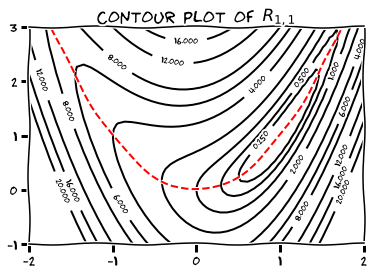
\includegraphics[width=0.5\linewidth]{rosenbrockContour} &
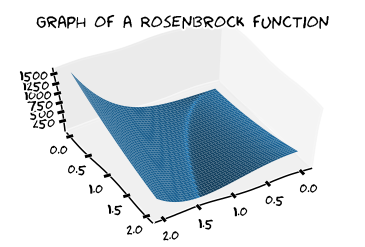
\includegraphics[width=0.5\linewidth]{rosenbrockGraph}
\end{tabular}
\caption{Details of the graph of $\mathcal{R}_{1,1}$}
\label{figure:Rosenbrock}
\end{figure}
It is also easy to verify that the image is the interval $[0,\infty)$.  Indeed, note first that $\mathcal{R}_{a,b}(x,y) \geq 0$ for all $(x,y) \in \field{R}^2$.  Zero is attained: $\mathcal{R}_{a,b} (a,a^2) = 0$.  Note also that $\mathcal{R}_{a,b}(0,y) = a^2 + by^2$ is a polynomial of degree 2, therefore unbounded.

Let's locate all local minima:
\begin{itemize}
	\item The gradient and Hessian are given respectively by
	\begin{equation*}
	\gradient{\mathcal{R}_{a,b}}(x,y) = \big[ 2(x-a) +4bx(x^2-y) , b(y-x^2) \big] \\
	\end{equation*}
	\begin{equation*}
	\Hess{\mathcal{R}_{a,b}}(x,y) = \begin{bmatrix}
	12bx^2-4by+2 & -4bx \\
	-4bx & 2b
	\end{bmatrix}
	\end{equation*}
	\item The search for critical points $\gradient{\mathcal{R}_{a,b}} = \boldsymbol{0}$ gives only the point $(a,a^2)$. (Why?)
	\item $\frac{\partial^2 \mathcal{R}_{a,b}}{\partial x^2}(a,a^2) = 8ba^2+2 > 0$.
	\item The Hessian at that point has positive determinant:
	\begin{equation*}
	\det \Hess{\mathcal{R}_{a,b}}(a,a^2) = \det \begin{bmatrix}
	8ba^2+2 & -4ab \\
	-4ab & 2b
	\end{bmatrix} = 4b > 0
	\end{equation*}
\end{itemize}
There is only one local minimum at $(a,a^2)$.
\end{example}

The second step was the notion of \emph{global (or absolute) minima}: points $(x_0,y_0)$ that satisfy $f(x_0,y_0) \leq f(x,y)$ for any point $(x,y)$ in the domain of $f$.  We always started with the easier setting, in which we placed restrictions on the domain of our functions:

\begin{theorem}\label{theorem:MaxMinCompact}
A continuous real-valued function always attains its minimum value on a \emph{compact} set $K$. To search for global minima, we perform the following steps:
\begin{description}
	\item[Interior Candidates] List the critical points of $f$ located in the interior of $K$.
	\item[Boundary Candidates] List the points in the boundary of $K$ where $f$ may have minimum values.
	\item [Evaluation/Selection] Evaluate $f$ at all candidates and select the one(s) with the smallest value.
\end{description}
\end{theorem}

\begin{example}
A flat circular plate has the shape of the region $x^2+y^2 \leq 1$. The plate, including the boundary, is heated so that the temperature at the point $(x,y)$ is given $T(x,y) =x^2 +2 y^2 - x$.  Find the temperature at the coldest point of the plate.

We start by searching for critical points.  The equation $\gradient{f}(x,y) = 0$ gives $x=\tfrac{1}{2}$, $y=0$. The point $\big(\tfrac{1}{2}, 0\big)$ is clearly inside of the plate.  This is our first candidate.

The border of the plate can be parameterized by $\varphi(t) = (\cos t, \sin t)$ for $t \in [0,2\pi)$.  The search for minima in the boundary of the plate can then be coded as an optimization problem for the function $h(t) = f \circ \varphi (t) = \cos^2 t + 2\sin^2 t - \cos t$ on the interval $[0,2]$.  Note that $h'(t) = 0$ at $t \in \{ 0, \tfrac{2}{3}\pi \}$ in $[0,2\pi]$.  We thus have two more candidates: 
\begin{equation*}
\varphi(0) = (1,0) \qquad \varphi\big(\tfrac{2}{3}\pi\big)= \big( -\tfrac{1}{2}, \tfrac{1}{2}\sqrt{3} \big)
\end{equation*}
Evaluation of the function at all candidates gives us the answer: $T\big( \tfrac{1}{2}, 0 \big) = -0.25$.
\end{example}

\section{Exercises}
\begin{problem}\label{problem:maxima}
Develop similar statements as in Definition \ref{def:localminimum}, Theorems \ref{theorem:localminimum}, \ref{theorem:2DTforLEV} and \ref{theorem:MaxMinCompact}, but for \emph{local} and \emph{global maxima}.
\end{problem}

\begin{problem}[Domains]
Find and sketch the domain of the following functions.
\begin{enumerate}
	\item $f(x,y) = \sqrt{y-x-2}$
	\item $f(x,y) = \log \big( x^2+y^2-4 \big)$
	\item $f(x,y) = \frac{(x-1)(y+2)}{(y-x)(y-x^3)}$
	\item $f(x,y) = \log (xy+x-y-1)$
\end{enumerate}
\end{problem}

\begin{problem}[Contour plots]
Find and sketch the level lines $f(x,y)=c$ on the same set of coordinate axes for the given values of $c$.
\begin{enumerate}
	\item $f(x,y) = x+y-1$, $c \in \{ -3, -2, -1, 0, 1, 2, 3\}$.
	\item $f(x,y) = x^2+y^2$, $c \in \{ 0, 1, 4, 9, 16, 25 \}$.
	\item $f(x,y) = xy$, $c \in \{ -9, -4, -1, 0, 1, 4, 9 \}$
\end{enumerate}
\end{problem}

\begin{problem}\label{problem:countours}
Use a Computer Algebra System of your choice (or script from your favorite computer language) to produce contour plots of the given functions on the given domains.
\begin{enumerate}
	\item $f(x,y) = (\cos x)(\cos y) e^{-\sqrt{x^2+y^2}/4}$ on $[-2\pi, 2\pi]\times [-2\pi, 2\pi]$.
	\item $g(x,y) = \dfrac{xy(x^2-y^2)}{x^2+y^2}$ on $[-1,1] \times [-1,1]$
	\item $h(x,y) = y^2 - y^4 -x^2$ on $[-1,1]\times[-1,1]$
\end{enumerate}
\begin{figure}[ht!]
\begin{tabular}{ccc}
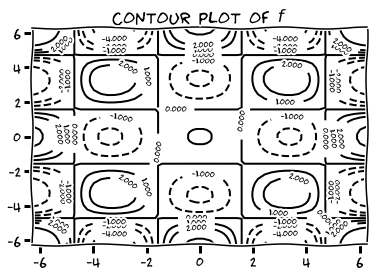
\includegraphics[width=0.33\linewidth]{contourf.png} &
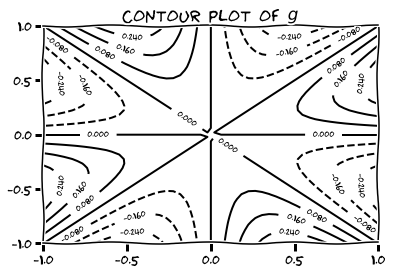
\includegraphics[width=0.33\linewidth]{contourg.png} &
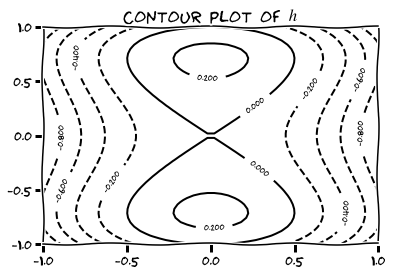
\includegraphics[width=0.33\linewidth]{contourh.png}
\end{tabular}
\caption{Contour Plots for problem \ref{problem:countours}}
\end{figure}
\end{problem}

\begin{problem} % example 2, p.858 in Thomas' Calculus
Find the points of the hyperbolic cylinder $x^2=z^2-1=0$ in $\field{R}^3$ that are closest to the origin.
\end{problem}